\subsection{Managing Hardware Failures}

<< REMOVE SECTION? >>
Another key issue with multi-core processing is the risk of hardware failure interrupting simulation runs. The increased number of cores, often spread out across multiple motherboards with individual power supplies, RAM and other components, leads to a much higher number of areas where a failure may occur. As the entire system is dependant on all utilized cores running in tandem, steps must be taken to mitigate this. 

One option is through core redundancy, where several cores run the same data, so the system is only interrupted when all cores running a specific data set fail. While this is simple in theory, it creates substantial problems of its own. For example, as simulations often make use of all available computing power there would be a limit on the simulation scale equal to the number of copies being ran, reducing data resolution. There is also the issue having to decide which result is "correct" for each individual data set when machine precision errors could cause them to marginally differ. 

Alternatively, the simulation can create regular data dumps, or checkpoints, that allow for the simulation to be resumed in the event of a hardware failure or other similar problem. These checkpoints require all variables, even those only used temporarily such as values derived from previous steps, to be dumped so that when loaded, the simulation can return to an identical state to that when the checkpoint was created and thus continue unaffected. Due to the size that these files can reach as well as the time required to save the data to disk, it is ill advised to create checkpoints for every timestep in the simulation. Instead, a balance must be found between reducing the possible data loss from a failure and limiting the data storage and computational costs of a high rate of checkpointing.


* http://charmplusplus.org/tutorial/CharmConcepts.html helpful

* Each core is allocated a tree piece

* Each tree piece has subset of binary tree

* All tree pieces have access to properties of root node

* Each tree piece runs code in serial

\iffalse


A simple system of two particles in a uniform, optically thin medium was created as shown in figure \ref{fig:complexSource}. The flux of all sink particles was calculated using an opening angle of 0.3. 
\begin{figure} [H]
    \centering
    \includegraphics[width=\textwidth]{plots/CH4/csICs.pdf}
    \caption{Plot of the initial conditions of the test for angular variation in complex sources}
    \label{fig:complexSource}
\end{figure}
Figure \ref{fig:complexSourceAngleVariation} shows the variation in error as a function of the angle between the particle and the $x$ axis of all particles within 1 smoothing length of the $z=0$ plane. The error caused by the merging of the cells is clear, with variation of up to 50\% of the minimum value for the unmerged sources. 
\begin{figure} [H]
    \centering
    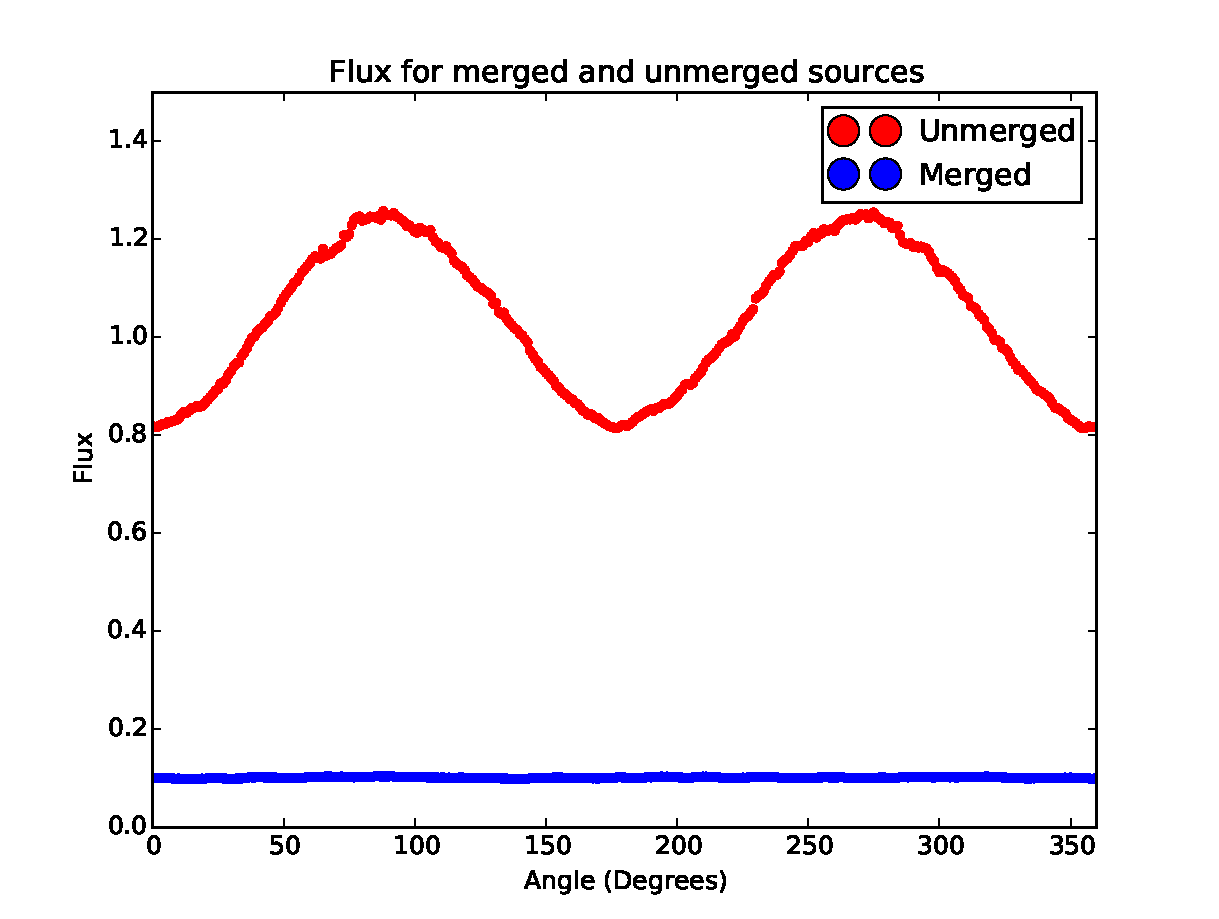
\includegraphics[width=\textwidth]{plots/CH4/csFlux.pdf}
    \caption{Flux as a function of angle of both the merged and unmerged sources}
    \label{fig:complexSourceAngleVariation}
\end{figure}
Another feature of this system is the "Lighthouse" effect. By increasing the opacity of the gas particles, the angles where the flux is at a minimum increase in range, limiting the region where the sources are visible. Figure \ref{fig:complexSourceLighthouseNormalized} shows a normalized plot of the flux of this system with varying opacity. The data was normalized by subtracting the minimum flux and dividing by the difference between the minimum and maximum flux and allows for the lighthouse effect to be seen regardless of the decrease in flux for the higher opacities. This effect is minimal at the optically thin limit and while maximized at the optically thick limit, the percentage flux that would penetrate the optically thick region is so low that the impact on accuracy is negligible. 
\begin{figure} [H]
    \centering
    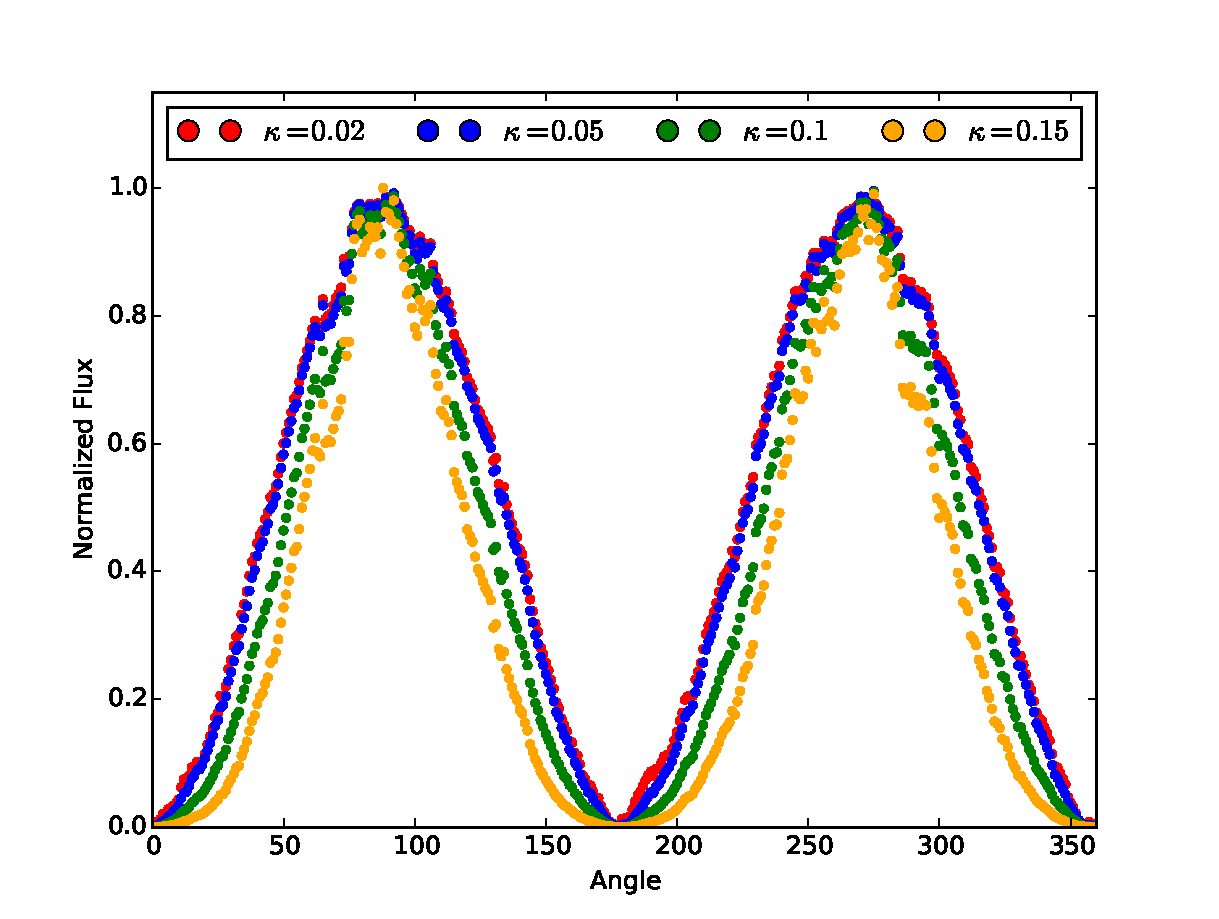
\includegraphics[width=\textwidth]{plots/CH4/csLighthouseNormalized.pdf}
    \caption{Normalized flux as a function of angle of the inner ring with varying opacities for the central gas sphere, showing the "lighthouse" effect}
    \label{fig:complexSourceLighthouseNormalized}
\end{figure}

This highlights the need for an accurate method for resolving complex sources in systems where the optical depth cannot be effectively estimated through the optically thick or thin limits.
\fi


This gives us

\begin{equation}
    \frac{D\rho}{Dt} + \rho \bigtriangledown \cdot v = 0
\end{equation}
\begin{equation}
    \rho \frac{Dv}{Dt} = -\bigtriangledown P + \frac{1}{c} \chi_F F
\end{equation}
\begin{equation}
    \rho \frac{D}{Dt} \bigg( \frac{E}{\rho} \bigg) = -\bigtriangledown \cdot F - \bigtriangledown v : P + 4\pi \kappa_p B -  c \kappa_E E
    \label{dyadic}
\end{equation}
\begin{equation}
    \rho \frac{D}{Dt} \bigg( \frac{e}{\rho} \bigg) = P \bigtriangledown \cdot v - 4 \pi \kappa_P B + c\kappa_E E
\end{equation}
\begin{equation}
        \frac{\rho}{c^2} \frac{D}{Dt} \bigg( \frac{F}{\rho} \bigg) = - \bigtriangledown \cdot P - \frac{1}{c} \chi_F F
\end{equation}

where $\frac{D}{Dt} = \frac{\delta}{\delta t} + v \cdot \bigtriangledown$, $\rho$, e, v and p are the mass density, energy density, velocity and pressure and E, F and P are the radiation energy density, the flux and the pressure tensor respectively. The three opacity terms, $\chi_F, \kappa_p$ and $\kappa_E$, give the total opacity, Planck mean absorption opacity and energy mean absorption opacity respectively. B is the Planck function and c is the speed of light. Equation \ref{dyadic} includes dyadic notation, allowing for the second order tensor $P$ to be written in vector algebra form.
